
\title{Lecture 10\\Representation of Correspondences in a Knowledge Base}

\begin{frame}
	\titlepage
\end{frame}

\begin{frame}{\\Lecture outline}
	\topline
	\justifying
	Types of correspondences. Single-valued and multivalued correspondences. Domain and codomain of a correspondence; image and preimage. Mappings and bijective correspondences. Correspondences between structures. Homomorphisms, isomorphisms and automorphisms; representation in a knowledge base.
\end{frame}

\begin{frame}{\\Types of correspondences}
\topline
\begin{SCn}
\scnheader{correspondence*}
\scnidtf{existence of a correspondence*}
\begin{scnrelfromset}{partition}
        \scnitem{single-valued correspondence*}
	\scnitem{multivalued correspondence*}
\end{scnrelfromset}
\begin{scnrelfromset}{partition}
        \scnitem{total correspondence*}
	\scnitem{partial correspondence*}
\end{scnrelfromset}
\begin{scnrelfromset}{partition}
        \scnitem{surjection*}
	\scnitem{non-surjective correspondence*}
\end{scnrelfromset}
\end{SCn}
\end{frame}

\begin{frame}{\\Single-valued correspondence}
\topline
\begin{SCn}
\scnheader{single-valued correspondence*}
\scnidtf{existence of a single-valued correspondence*}
\scnidtf{functional correspondence*}
\scnidtf{function*}
    \scnrelfrom{definition}{\normalfont{[} single-valued correspondence* is a correspondence* in which each element of the source set is associated with at most one element of the target set.\normalfont{]}}
\end{SCn}
\end{frame}

\begin{frame}{\\Single-valued correspondence}
    \topline
    \begin{center}
        \begin{figure}[Hb]
            \centering
            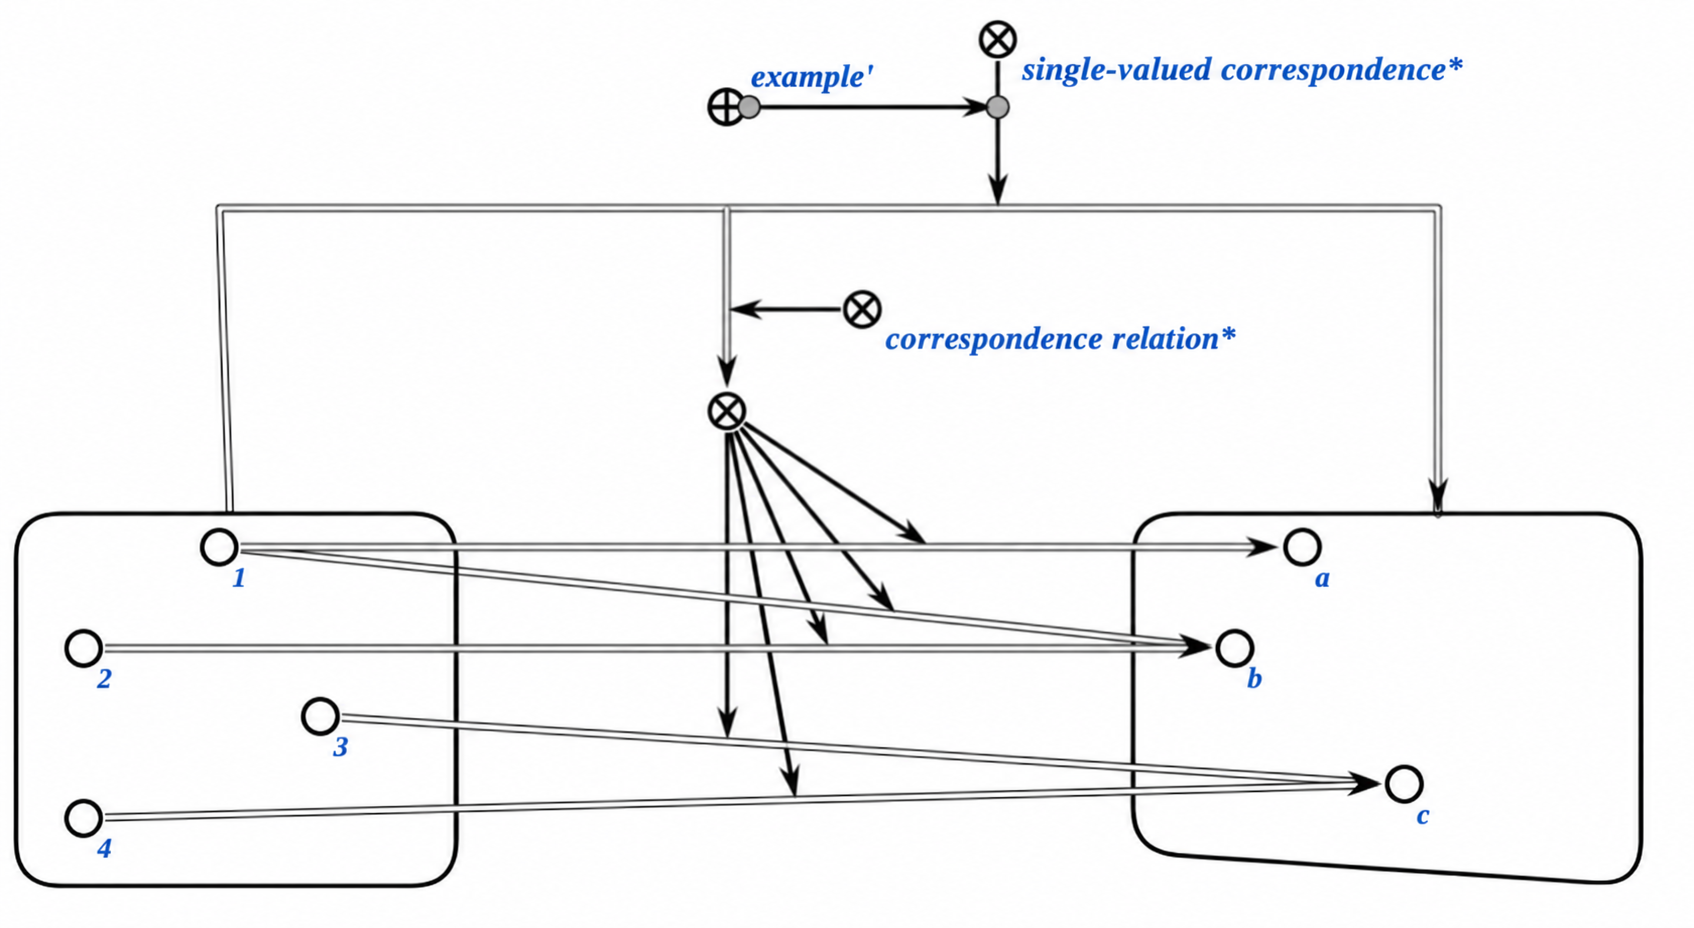
\includegraphics[width=324.8bp,height=178.0bp,keepaspectratio]{figures/sd_correspondences/One-to-one correspondence_en.png}
        \end{figure}
    \end{center}
\end{frame}

\begin{frame}{\\Multivalued correspondence}
\topline
\begin{SCn}
\scnheader{multivalued correspondence*}
\scnrelfrom{definition}{\normalfont{[} multivalued correspondence* is a correspondence* in which at least one element of the source set is associated with more than one element of the target set.\normalfont{]}}
\end{SCn}
\end{frame}

\begin{frame}{\\Multivalued correspondence}
    \topline
    \begin{center}
        \begin{figure}[Hb]
            \centering
            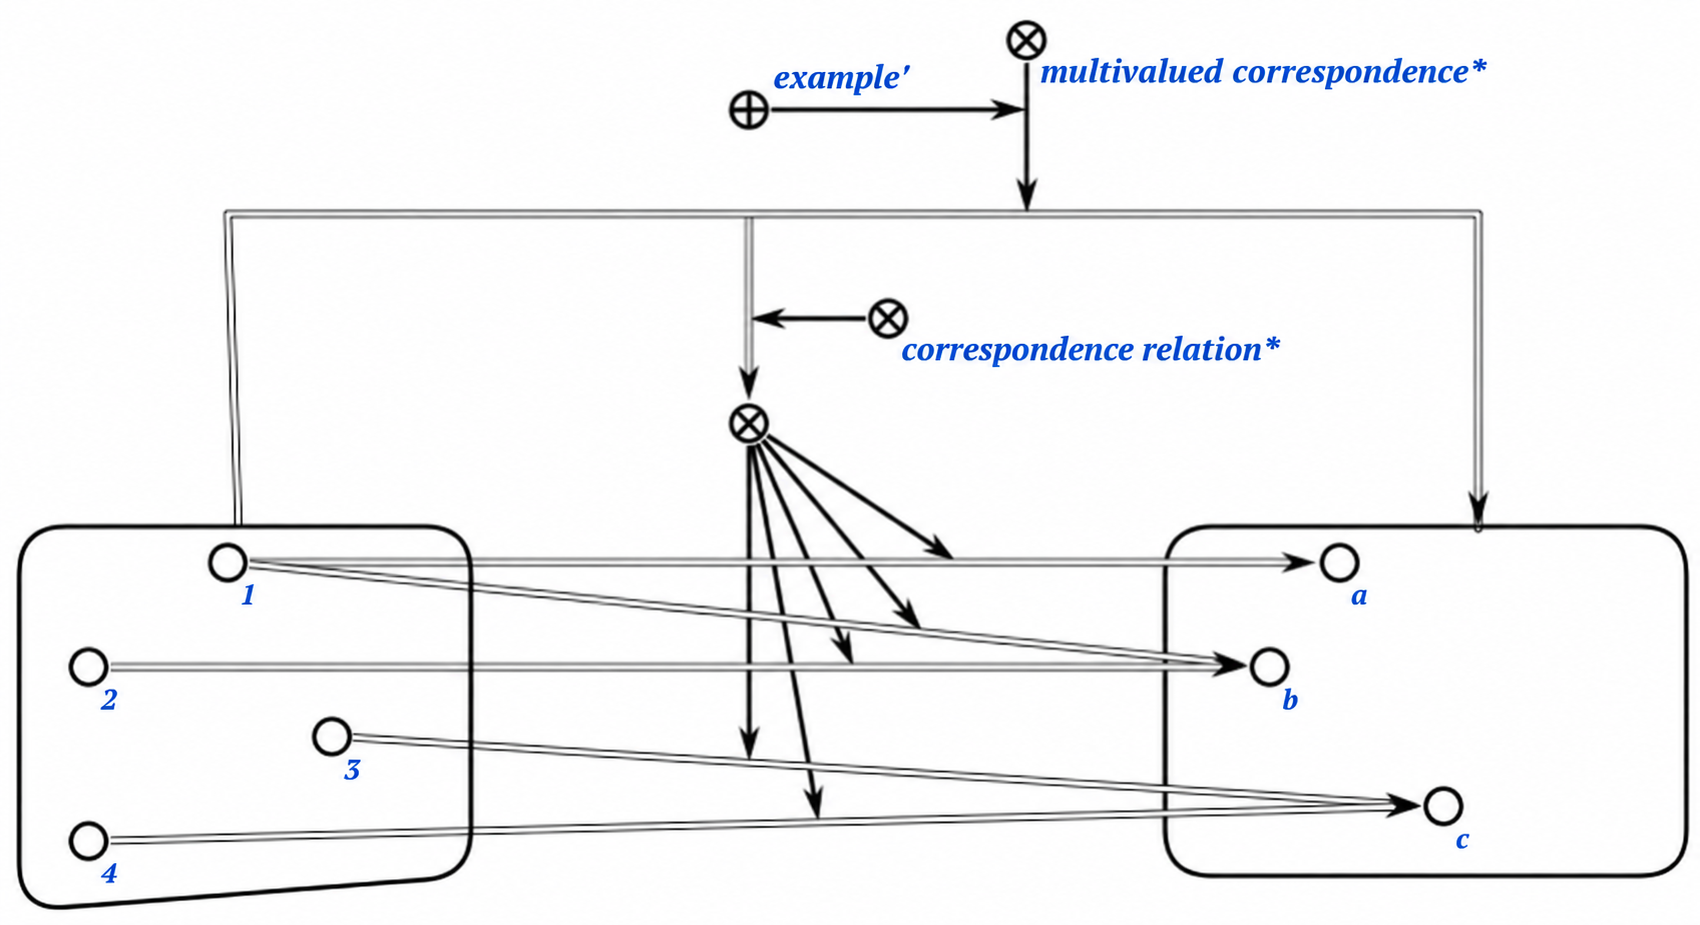
\includegraphics[width=317.5bp,height=172.8bp,keepaspectratio]{figures/sd_correspondences/Ambiguous correspondence_en.png}
        \end{figure}
    \end{center}
\end{frame}

\begin{frame}{\\Domain of a correspondence}
\topline
\begin{SCn}
\scnheader{domain of a correspondence\scnrolesign}
\scnidtf{source set of a correspondence\scnrolesign}
\scnidtf{first component of a pair in the correspondence relation\scnrolesign}
\scniselement{role relation}
\scnrelfrom{definition}{\normalfont{[} domain of a correspondence\scnrolesign is a role relation that identifies the first component of a pair in the correspondence* relation.\normalfont{]}}
\end{SCn}
\end{frame}

\begin{frame}{\\Codomain of a correspondence}
\topline
\begin{SCn}
\scnheader{codomain of a correspondence\scnrolesign}
\scnidtf{target set of a correspondence\scnrolesign}
\scnidtf{second component of a pair in the correspondence relation\scnrolesign}
\scniselement{role relation}
\scnrelfrom{definition}{\normalfont{[} target set is a role relation that identifies the second component of a pair in the correspondence* relation\normalfont{]}}
\end{SCn}
\end{frame}

\begin{frame}{\\Image of a correspondence}
\topline
\begin{SCn}
\scnheader{image\scnrolesign}
\scnidtf{image of a correspondence\scnrolesign}
\scniselement{role relation}
\scnidtf{second component of a pair in the correspondence relation\scnrolesign}
\scnrelfrom{definition}{\normalfont{[} image\scnrolesign is a role relation that identifies the second component of each pair in the set of pairs that is the second component of the correspondence* relation.\normalfont{]}}
\end{SCn}
\end{frame}

\begin{frame}{\\Preimage of a correspondence}
\topline
\begin{SCn}
\scnheader{preimage\scnrolesign}
\scnidtf{preimage of a correspondence\scnrolesign}
\scniselement{role relation}
\scnidtf{first component of a pair in the correspondence relation\scnrolesign}
\scnrelfrom{definition}{\normalfont{[} preimage\scnrolesign is a role relation that identifies the first component of each pair in the set of pairs that is the first component of the correspondence* relation.\normalfont{]}
}
\end{SCn}
\end{frame}

\begin{frame}{\\Mapping}
\topline
\begin{SCn}
\scnheader{mapping*}
\scnsubset{total correspondence*}
\scnsubset{single-valued correspondence*}
\scnrelfrom{definition}{\normalfont{[} mapping* is a single-valued total correspondence.\normalfont{]}
}
\end{SCn}
\end{frame}

\begin{frame}{\\Mapping}
    \topline
    \begin{center}
        \begin{figure}[Hb]
            \centering
            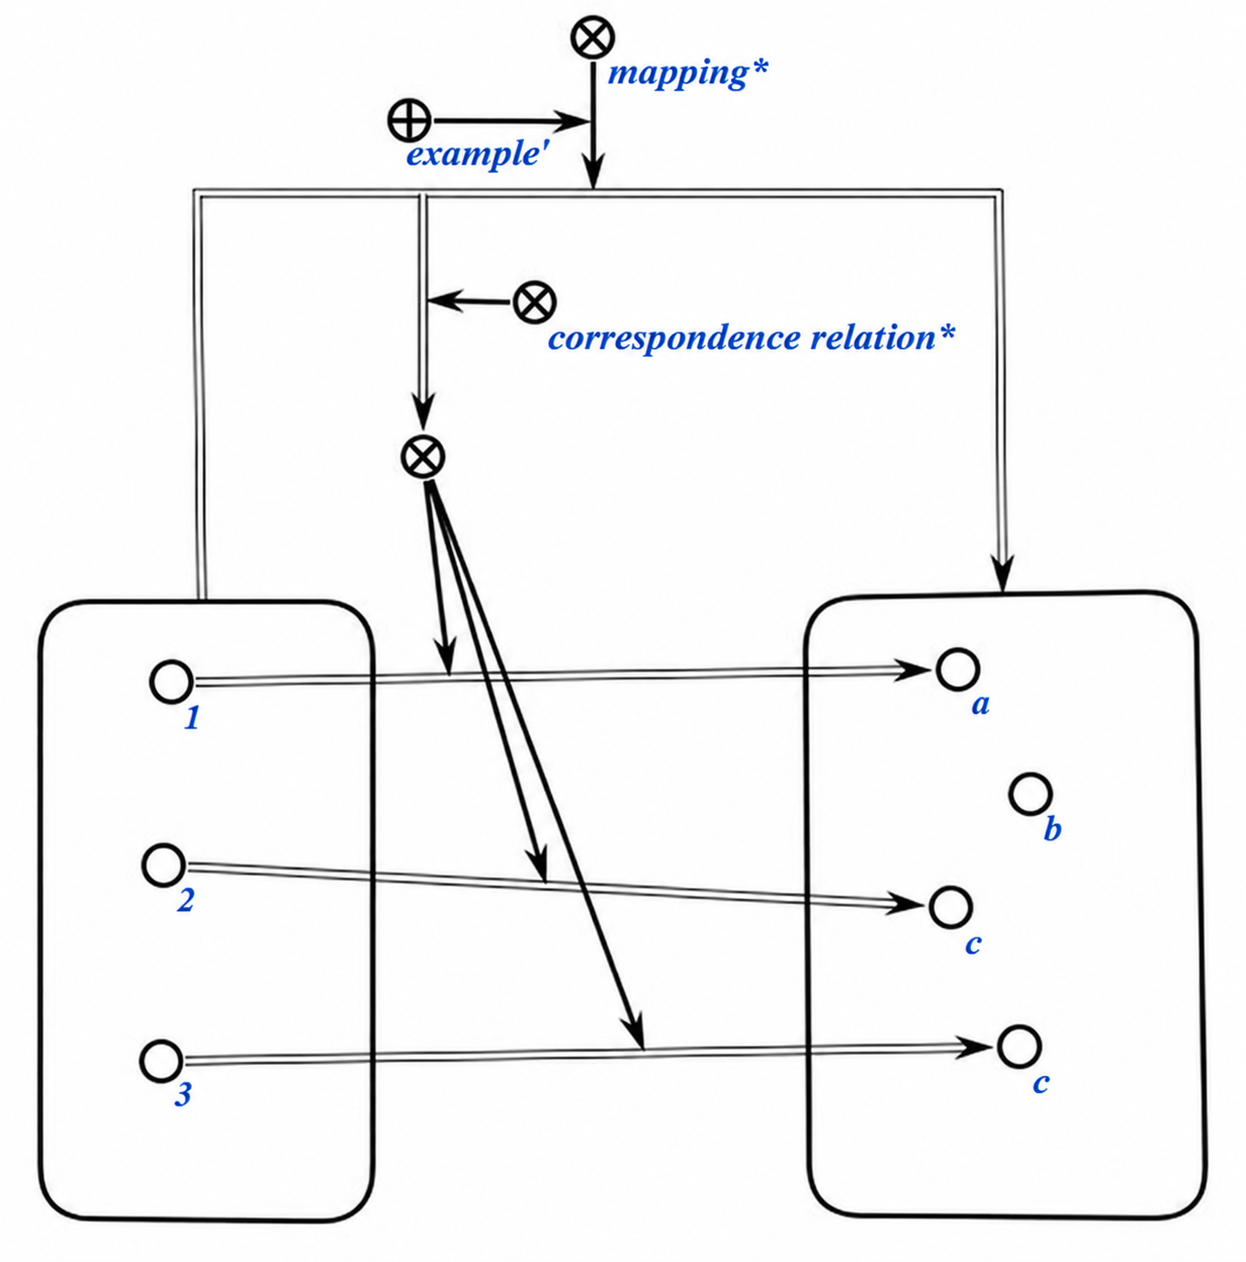
\includegraphics[width=163.0bp,height=165.0bp,keepaspectratio]{figures/sd_correspondences/Display_en.png}
        \end{figure}
    \end{center}
\end{frame}

\begin{frame}{\\Bijective correspondence}
\topline
\begin{SCn}
\scnheader{bijective correspondence*}
\scnidtf{bijection*}
\scnidtf{one-to-one correspondence*}
\scnsubset{total correspondence*}
\scnsubset{single-valued correspondence*}
\scnsubset{surjective correspondence*}
\scnrelfrom{definition}{\normalfont{[} bijective correspondence* is a single-valued, total, surjective correspondence.\normalfont{]}
}
\end{SCn}
\end{frame}

\begin{frame}{\\Bijective correspondence}
    \topline
    \begin{center}
        \begin{figure}[Hb]
            \centering
            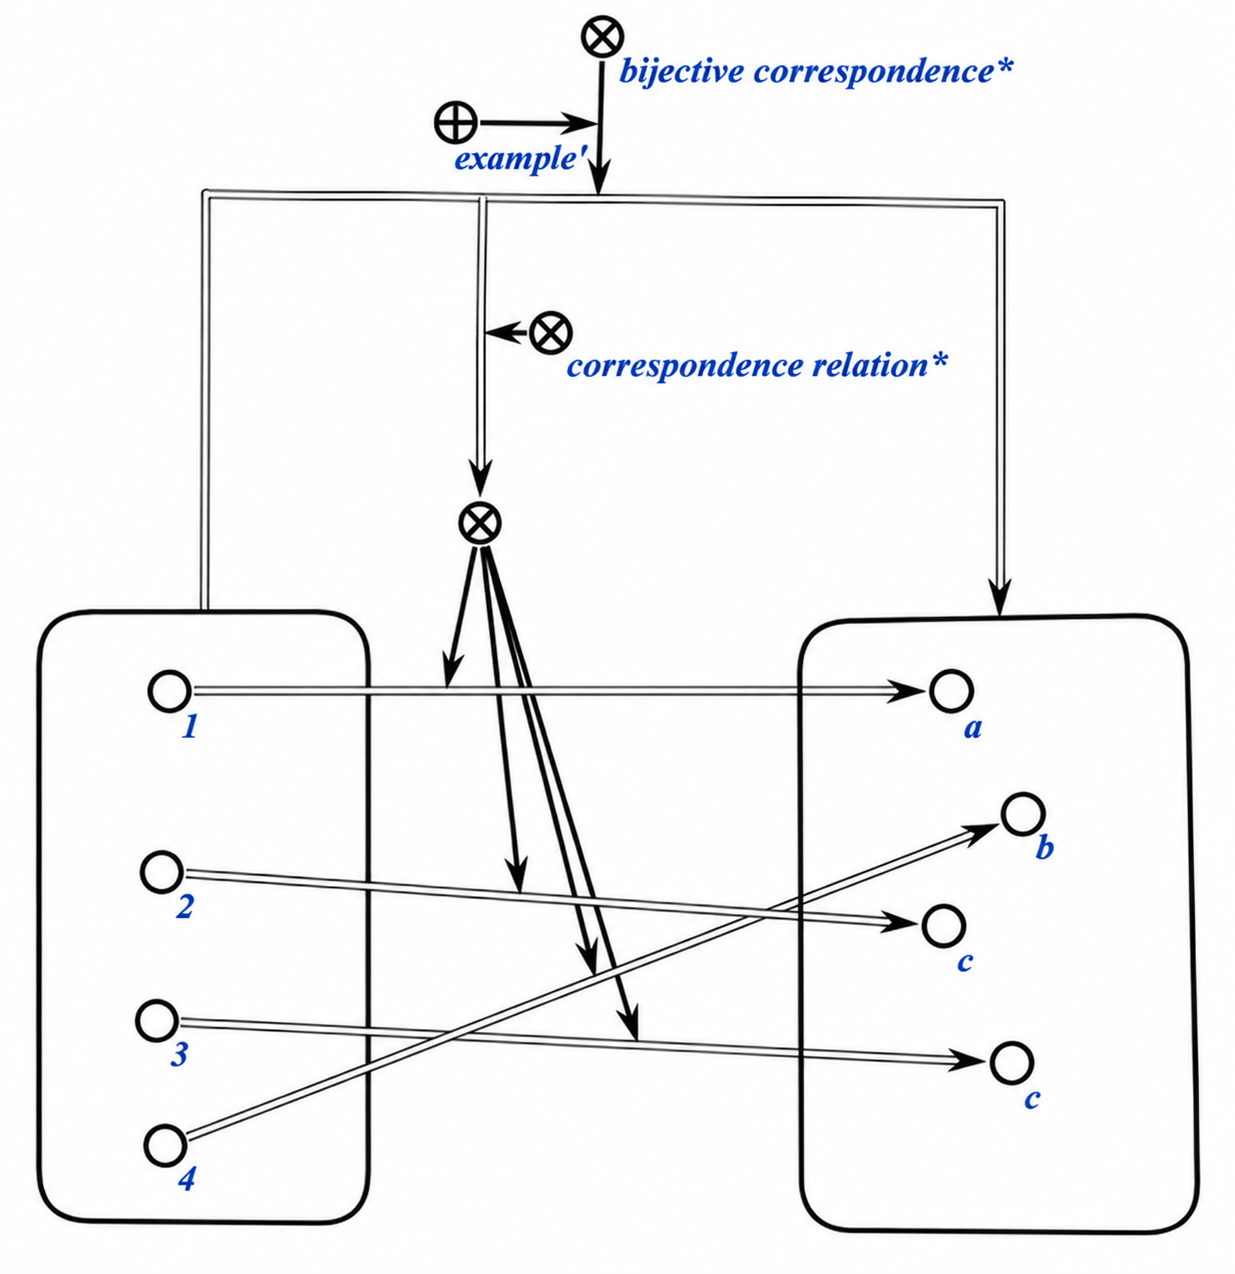
\includegraphics[width=163.7bp,height=168.7bp,keepaspectratio]{figures/sd_correspondences/Bijection_en.png}
        \end{figure}
    \end{center}
\end{frame}

\begin{frame}{\\Correspondences between structures}
\topline
\begin{SCn}
A structure is a set of sc-elements such that removing one of them may violate the integrity of the set.

Several types of correspondences can be defined between structures, including \textbf{homomorphism, automorphism and isomorphism}, as well as structural analogy, which allows us to record an analogy,
similarities and differences between substructures of the structures under consideration.
\end{SCn}
\end{frame}

\begin{frame}{\\Homomorphism}
\topline
\begin{SCn}
\scnheader{homomorphism relation*}
\scnidtf{homomorphism relation between structures*}
\scnsubset{correspondence*}
\scniselement{binary relation}
\scnrelfrom{explanation}{\normalfont{[} homomorphism relation* is a correspondence between structures in which each element of the domain (the first structure) is associated with exactly one element of the codomain (the second structure).\normalfont{]}}

\scnheader{homomorphism*}
\scniselement{binary relation}
\end{SCn}
\end{frame}

\begin{frame}{\\Homomorphism}
    \topline
    \begin{center}
        \begin{figure}[b]
            \centering
            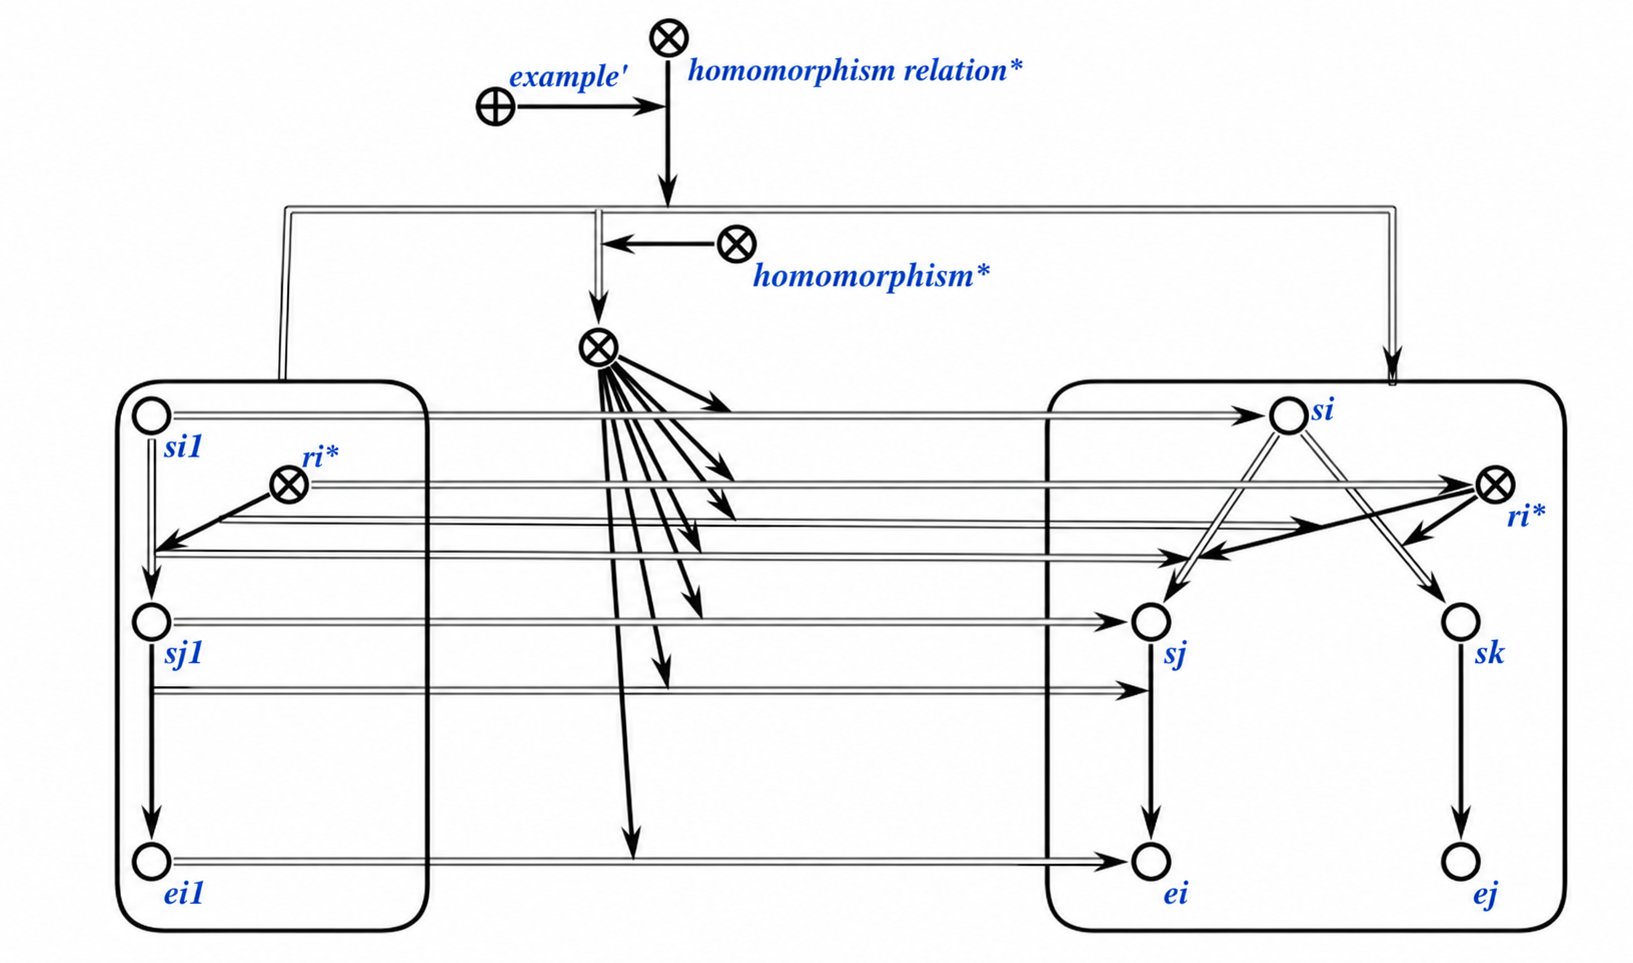
\includegraphics[width=281.6bp,height=166.0bp,keepaspectratio]{figures/sd_correspondences/Homomorphism_en.png}
        \end{figure}
    \end{center}
\end{frame}

\begin{frame}{\\Isomorphism}
\topline
\begin{SCn}
\scnheader{isomorphism relation*}
\scnidtf{isomorphism relation between structures*}
\scnsubset{correspondence*}
\scniselement{binary relation}
\scnrelfrom{explanation}{\normalfont{[} isomorphism relation* is a homomorphism relation* in which every element of the codomain has exactly one corresponding element in the domain.\normalfont{]}}

\scnheader{isomorphism*}
\scniselement{binary relation}
\end{SCn}
\end{frame}

\begin{frame}{\\Isomorphism}
    \topline
    \begin{center}
        \begin{figure}[b]
            \centering
            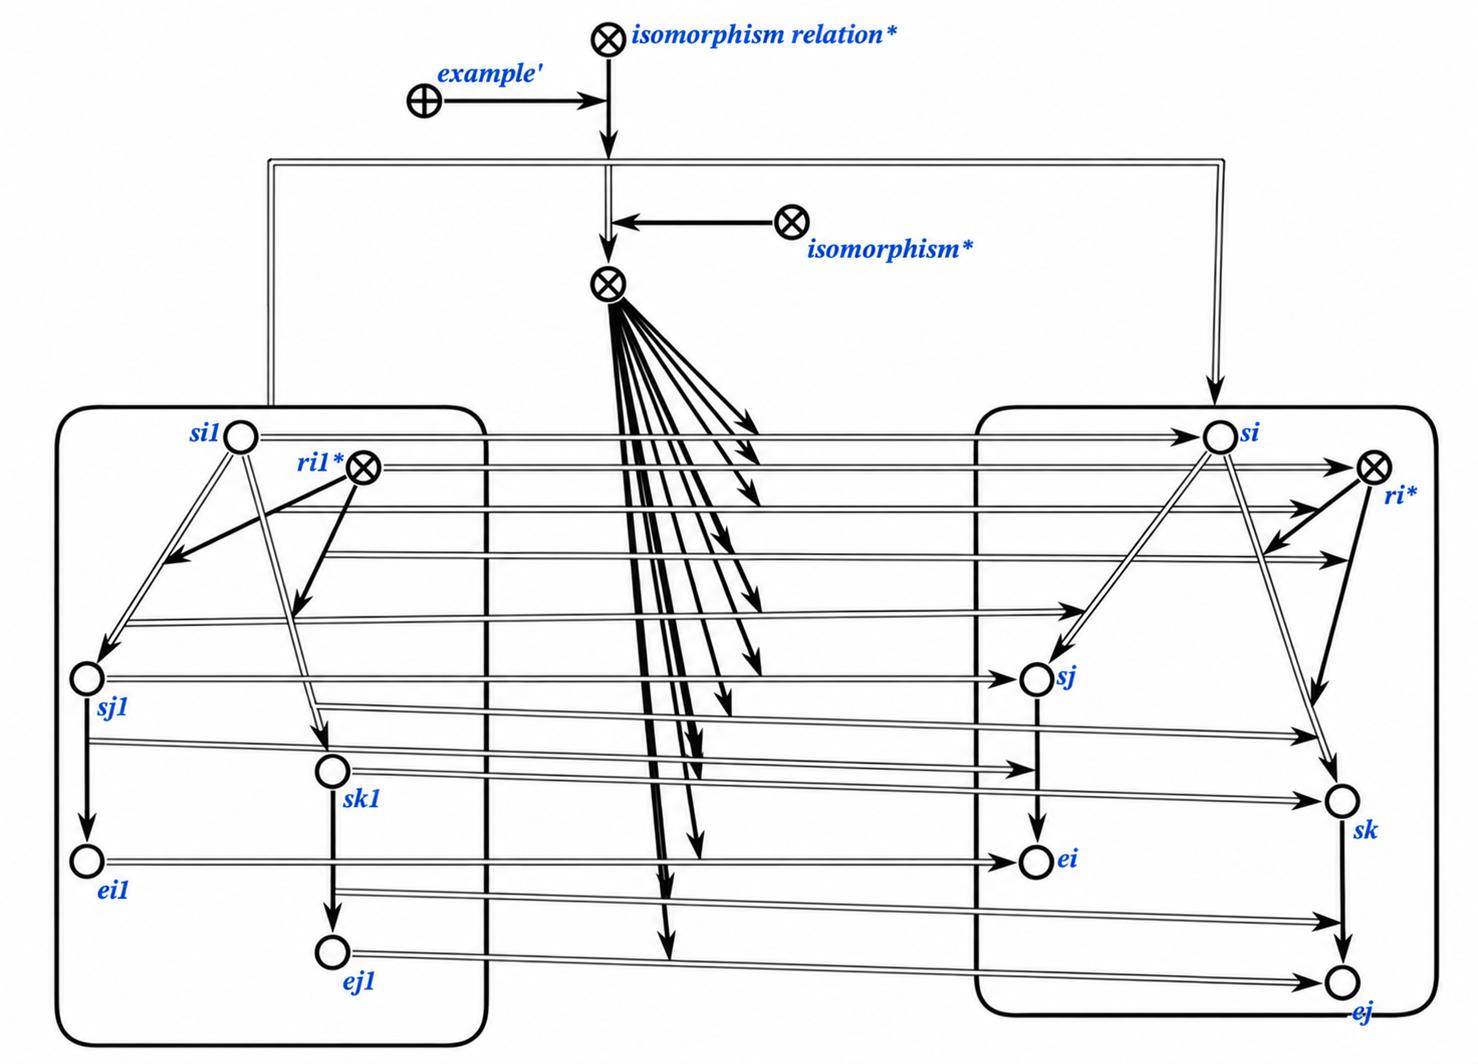
\includegraphics[width=239.1bp,height=171.9bp,keepaspectratio]{figures/sd_correspondences/Isomorphism_en.png}
        \end{figure}
    \end{center}
\end{frame}

\begin{frame}{\\Automorphism}
\topline
\begin{SCn}
\scnheader{automorphism relation*}
\scnidtf{automorphism relation between structures*}
\scnsubset{correspondence*}
\scniselement{binary relation}
\scnrelfrom{explanation}{\normalfont{[} automorphism relation* is an isomorphism relation* whose domain and codomain coincide.\normalfont{]}}

\scnheader{automorphism*}
\scniselement{binary relation}
\end{SCn}
\end{frame}

\begin{frame}{\\Automorphism}
    \topline
    \begin{center}
        \begin{figure}[b]
            \centering
            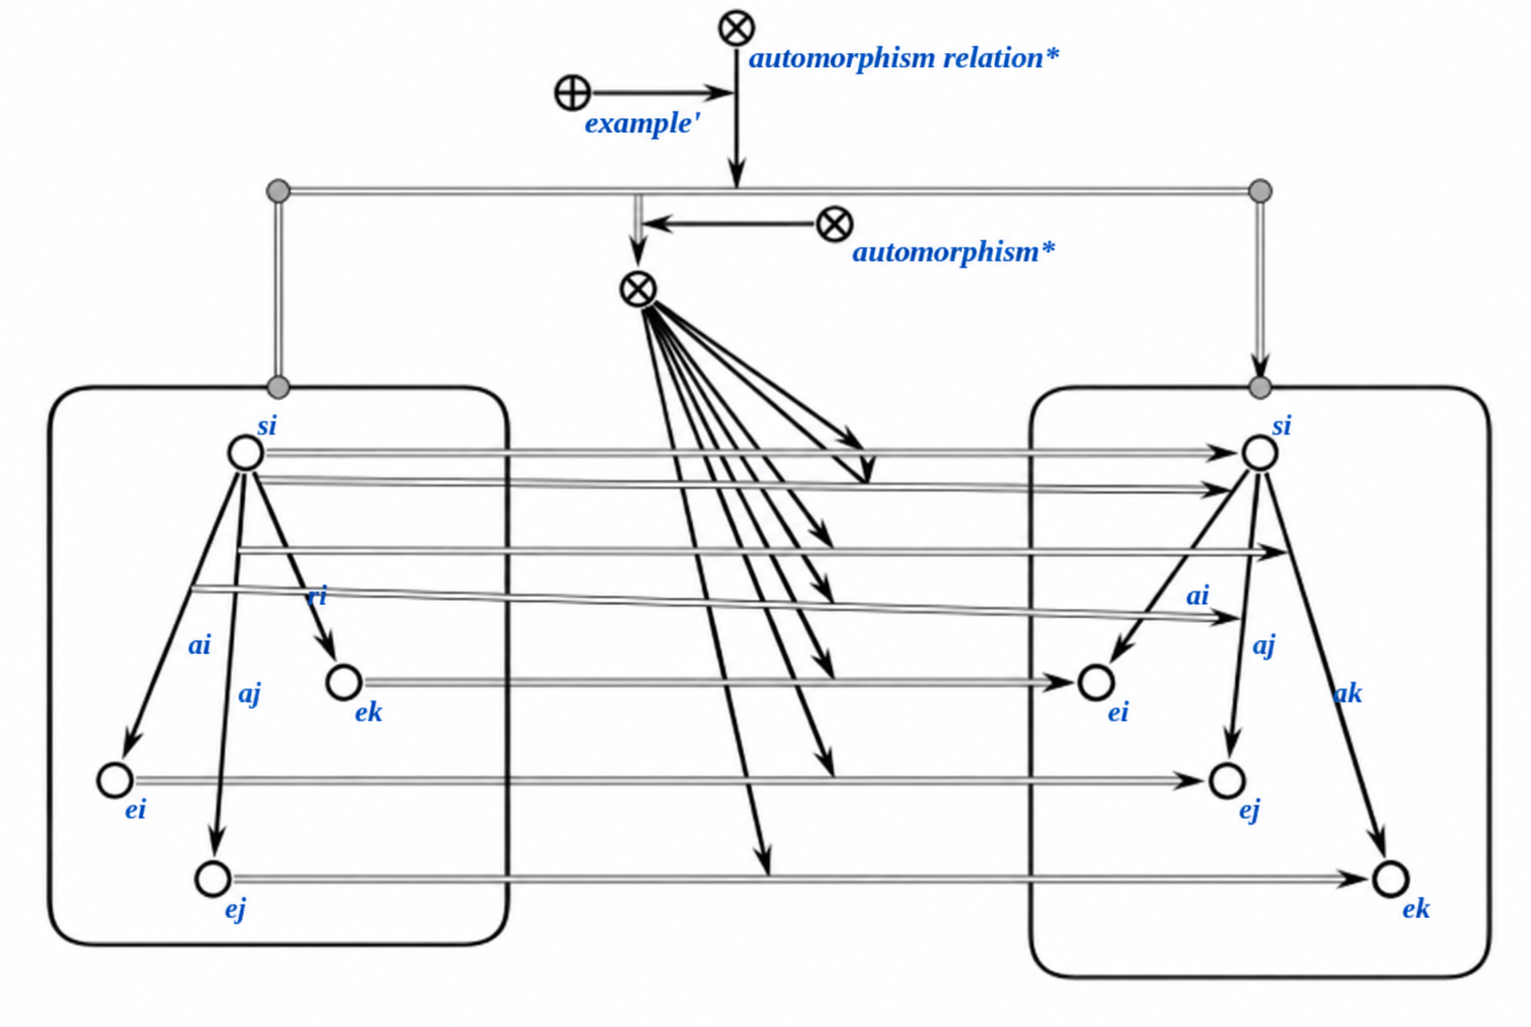
\includegraphics[width=254.8bp,height=170.9bp,keepaspectratio]{figures/sd_correspondences/Automorphism_en.png}
        \end{figure}
    \end{center}
\end{frame}
